\documentclass{beamer}
\special{landscape}

\usetheme{Warsaw}

%\usecolortheme{seahorse}
%\usefonttheme[onlysmall]{structurebold}

\setbeamertemplate{headline}[split]
\setbeamertemplate{footline}[default]
\setbeamertemplate{footline}[miniframes theme]
%\logo{\includegraphics[scale=0.25]{lifia_logo.png}}

\mode<presentation>
\usepackage[spanish]{babel}
\usepackage{beamerthemesplit}
\usepackage{color}      % use if color is used in text

\usepackage[utf8]{inputenc}

% Comandos en modo Verbatim
%\usepackage{fancyvrb}

\usepackage{listings}


\lstdefinelanguage[mips]{Assembler}{%
  sensitive=false,%
  morecomment=[l]{;},%
  % so listings can detect directives and register names
  alsoletter={.\$},
  % strings, characters, and comments
  morestring=[b]",
  morestring=[b]',
  morecomment=[l]\#,
  numberstyle=\color{green},
  % instructions
  morekeywords={[1]cvt.l.d,cvt.d.l,mfc1,mtc1,DADD,DADDI,ANDI,XORI,HALT,BEQ,BNEQ,LD,NOP,DMUL,DSUB,AND,DDIV,%
	JAL,J,DSLL,BNEZ,SD, JR, BEQZ, cvt.d.l, cvt.l.d, lwu},
  % assembler directives
  morekeywords={[2].word,.code,.data, .asciiz, .ascii, .word32},
  % register names
  morekeywords={[3]F0,F1,F2,F3,F4,F5,F6,F7,F8,F9,F10,F11,F12,F13,F14,F15,F16,F17,F18,F19,%
    F20,F21,F22,F23,F24,F25,F26,F27,F28,F29,F30,F31,%
    f0,f1,f2,f3,f4,f5,f6,f7,f8,f9,f10,f11,f12,f13,f14,f15,f16,f17,f18,f19,%
    f20,f21,f22,f23,f24,f25,f26,f27,f28,f29,f30,f31,%
    R0,R1,R2,R3,R4,R5,R6,R7,R8,R9,R10,R11,R12,R13,R14,R15,R16,R17,R18,R19,%
    R20,R21,R22,R23,R24,R25,R26,R27,R28,R29,R30,R31,%
    r0,r1,r2,r3,r4,r5,r6,r7,r8,r9,r10,r11,r12,r13,r14,r15,r16,r17,r18,r19,%
    r20,r21,r22,r23,r24,r25,r26,r27,r28,r29,r30,r31,%
	\$0,\$zero,\$s0,$s1,$s2,$s3,$s4,$s5,$s6,$s7,$sp,$ra,$t0,$t1,$t2,$t3,$t4,$t5,$t6,$t7,$t8,$t9,%
	$sp,$a0,$a1,$a2,$a3,$v0,$v1%
    },
  keywordstyle=\color{green},
  keywordstyle=[2]\color{blue},% for example
  keywordstyle=[2]\color{blue},% for example
  keywordstyle=[3]\color{red},% for example
 }[strings,comments,keywords]


\definecolor{CommentGreen}{rgb}{0,.6,0}
\lstset{
   language=[mips]Assembler,
   escapechar=@, % include LaTeX code between `@' characters
   keepspaces,   % needed to preserve spacing with lstinline
   basicstyle=\footnotesize\ttfamily\bfseries,
   commentstyle=\color{CommentGreen},
   stringstyle=\color{cyan},
   showstringspaces=false,
   keywordstyle=[1]\color{blue},    % instructions
   keywordstyle=[2]\color{magenta}, % directives
   keywordstyle=[3]\color{red},     % registers
%  numbers=left,
%  numbersep=15pt,
%  numberstyle=\tiny\color{green},
 }

%%
%% WinMIPS64 definition (c) 2020
%\lstdefinelanguage{WinMIPS64_old}
% {keywords={%
%cvt.l.d,cvt.d.l,mfc1,mtc1,DADD,DADDI,ANDI,XORI,HALT,BEQ,BNEQ,LD,NOP,DMUL,DSUB,AND,DDIV,%
%	JAL,J,DSLL,BNEZ,SD, JR, BEQZ, cvt.d.l, cvt.l.d, lwu},%
% otherkeywords={.word,.code,.data,.code, .asciiz, .ascii, .word32 },%
%   sensitive=false,%
%   morecomment=[l]{;},%
%   morestring=[b]",%
%   keywordstyle=\color{green},
%  keywordstyle=[2]\color{brown},% for example
% }

%\lstset{emph={%
%    F0,F1,F2,F3,F4,F5,F6,F7,F8,F9,F10,F11,F12,F13,F14,F15,F16,F17,F18,F19,%
%    F20,F21,F22,F23,F24,F25,F26,F27,F28,F29,F30,F31,%
%    f0,f1,f2,f3,f4,f5,f6,f7,f8,f9,f10,f11,f12,f13,f14,f15,f16,f17,f18,f19,%
%    f20,f21,f22,f23,f24,f25,f26,f27,f28,f29,f30,f31,%
%    R0,R1,R2,R3,R4,R5,R6,R7,R8,R9,R10,R11,R12,R13,R14,R15,R16,R17,R18,R19,%
%    R20,R21,R22,R23,R24,R25,R26,R27,R28,R29,R30,R31,%
%    r0,r1,r2,r3,r4,r5,r6,r7,r8,r9,r10,r11,r12,r13,r14,r15,r16,r17,r18,r19,%
%    r20,r21,r22,r23,r24,r25,r26,r27,r28,r29,r30,r31,%
%	\$0,\$zero,\$s0,$s1,$s2,$s3,$s4,$s5,$s6,$s7,$sp,$ra,$t0,$t1,$t2,$t3,$t4,$t5,$t6,$t7,$t8,$t9,%
%	$sp,$a0,$a1,$a2,$a3,$v0,$v1%
%    },emphstyle={\color{red}\bfseries}%
%}%

%\lstset{emph={%
%    .code,.data,.word
%    },emphstyle={\color{green}\bfseries}%
%}%

\title{Practica 6 - WinMIPS64}
%\author{Juan Antonio Zubimendi\\azubimendi@lifia.info.unlp.edu.ar}

\AtBeginSection[]

\begin{document}

\section{Segmentación de Cause}

\begin{frame}
\frametitle{Segmentación de Cause}
\begin{itemize}
\item Si las etapas son independientes podemos ejecutarlas en paralelo
\item Mientras ejecutamos una etapa de una instrucción, ejecutamos otra etapa de otra instrucción.
\item De esta manera usamos mejor la CPU, todas las etapas estan en funcionamiento en cada ciclo de CPU.
\begin{itemize}
  \item Cada instrucción tarda en ejecutarse 5 ciclos
  \item $1$ instrucción, 5 ciclos
  \item $2$ instrucciones, 6 ciclos
  \item $3$ instrucciones, 7 ciclos
  \item $10$ instrucciones, 14 ciclos
  \item $n$ cantidad de instrucciones se ejecutaran en $4 + n$ ciclos.
\end{itemize}
\item A esta técnica se la llama Segmentación de Cause
\end{itemize}
\end{frame}


\subsection{Ciclo de Instrucción}
\begin{frame}
\frametitle{Ciclo de Instruccion de WinMIPS64}
\begin{itemize}
\item Busqueda (IF)
\begin{itemize}
  \item Se accede a la memoria buscando la instrucción
  \item Se incrementa el PC
\end{itemize}
\item Decodificación / Búsqueda de Operandos (ID)
\begin{itemize}
  \item Se decodifica la instrucción
  \item Se accede al banco de registro por los operandos en la segunda mitad del ciclo. No puede avanzar si no estan disponibles.
  \item Si es un salto condicional, se determina si hay que realizarlo o no
  \item Si hay que ejecutar un salto, también se calcula el nuevo PC
\end{itemize}
\item Ejecución / Dirección Efectiva (EX)
\begin{itemize}
  \item Si es una instrucción aritmetico/logica, se ejecuta en la ALU
  \item Si es acceso a memoria, se calcula la dirección efectiva
\end{itemize}
\item Acceso a Memoria (MEM)
\begin{itemize}
  \item Si es un acceso a memoria, se accede
\end{itemize}
\item Almacenamiento (WB)
\begin{itemize}
  \item Se almacena el resultado (si existiese) en el banco de registros en la primera mitad del ciclo
\end{itemize}
\end{itemize}
\end{frame}

\subsection{Diagrama}
\begin{frame}
\frametitle{}
\begin{itemize}
\item Cada etapa se ejecuta en un ciclo de reloj, salvo algunas operaciones aritmeticas de punto flotante, que tienen unidades de ejecuciión separadas
\item Las etapas de cada uniad de ejecución dependen de la operación a realizar:
\begin{itemize}
\item Suma (PF) se realiza en 4 ciclos, con 4 etapas
\item Multiplicación se realiza en 7 ciclos, con 7 etapas
\item División se realiza en 24 ciclos, 1 etapa
\end{itemize}
\item Distintas unidades de ejecución pueden estar activas al mismo tiempo
\end{itemize}
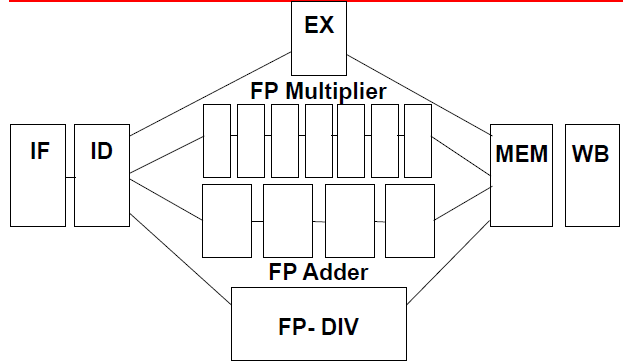
\includegraphics[scale=0.35]{ciclo-instruccion.png}
\end{frame}

\section{Atascos}

\subsection{Introducción}
\begin{frame}
\frametitle{Introducción}
Suposiciones:
\begin{itemize}
\item Todas las tareas duran el mismo tiempo.
\item Las instrucciones siempre pasan por todas las etapas.
\item Todos las etapas pueden ser manejadas en paralelo.
\end{itemize}
\end{frame}

\begin{frame}
\frametitle{Algunos Problemas}
Problemas:
\begin{itemize}
\item  No todas las instrucciones necesitan todas las etapas
\begin{itemize}
\item \emph{SW RT, inmed(RS)} -  no utiliza W
\item En VonSim \emph{MOV AX, mem} no requiere EX
\end{itemize}
 \item No todas las etapas pueden ser manejadas en paralelo.
\begin{itemize}
\item F y M acceden a memoria
\end{itemize}
\item No se tienen en cuenta los saltos de control.
\end{itemize}
\end{frame}


\begin{frame}
\frametitle{Atascos}
Llamamos \emph{atasco} a la situación que impide a una o mas instrucciones seguir su camino en el cauce.

Los atascos pueden ocurrir por 3 razones:

\begin{itemize}
\item Estructural
\begin{itemize}
\item Provocados por conflictos con los recursos.
\end{itemize}


\item Dependencia de Datos
\begin{itemize}
\item Dos instrucciones se comunican por medio de un dato
\end{itemize}

\item Dependencia de Control
\begin{itemize}
\item La ejecución de una instrucción depende de cómo se ejecute otra
\end{itemize}

\end{itemize}
Si resolvemos con paradas del cauce, disminuye el rendimiento
\end{frame}


\section{Atascos por dependencia de Datos}
\subsection{General}

\begin{frame}
\frametitle{Atasco por Dependencia de Datos}

Condición en la que los operandos fuente o destino de una instrucción no están disponibles en el momento en que se necesitan en una etapa determinada del cauce.
\begin{itemize}

\item Lectura después de Escritura (RAW, dependencia verdadera)
\begin{itemize}
\item  una instrucción genera un dato que lee otra posterior
\end{itemize}

\item Escritura después de Escritura (WAW, dependencia en salida)
\begin{itemize}
\item una instrucción escribe un dato después que otra posterior
\item sólo se da si se deja que las instrucciones se adelanten unas a otras
\end{itemize}

\item Escritura después de Lectura (WAR, antidependencia)
\begin{itemize}
\item una instrucción modifica un valor antes de que otra anterior que lo tiene que leer lo lea
\item Es el que menos suele darse
\end{itemize}
\end{itemize}
\end{frame}

\subsection{RAW - Lectura luego de una Lectura}
\begin{frame}[fragile]
\frametitle{RAW}
Una instrucción depende del resultado de otra instrucción que todavía no ha finalizado y debe esperar a que el resultado este disponible.
\begin{block}{}
\begin{lstlisting}[basicstyle=\ttfamily,keywordstyle=\color{blue}]
.code
LD   r1, 100(r2)
DADD r3, r1, r5
DSUB r5, r3, r6
AND  r7, r5, r9
\end{lstlisting}
\end{block}

\end{frame}

\begin{frame}[fragile]
\frametitle{RAW}
Una instrucción depende del resultado de otra instrucción que todavía no ha finalizado y debe esperar a que el resultado este disponible.
\begin{block}{}
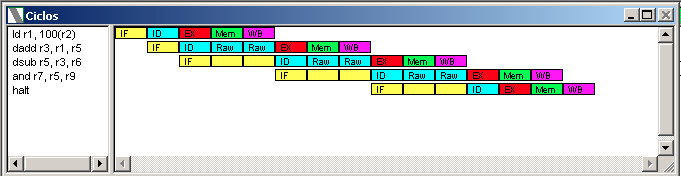
\includegraphics[scale=0.45]{raw.png}
\end{block}

\end{frame}



\section{Posibles soluciones a problemas de dependencia de datos}
\begin{frame}
\frametitle{General}
\begin{itemize}
\item Se debe determinar cómo y cuando aparecen esos riesgos
\item Hay dos tipos de soluciones
\begin{itemize}
\item Software
\begin{itemize}
\item Podemos agregar instrucciones \emph{NOP}, o reordenar las instrucciones
\end{itemize}
\item Hardware
\begin{itemize}
\item Adelantamiento de Operandos (Forwarding)
\end{itemize}
\end{itemize}
\end{itemize}
\end{frame}

\subsection{Agregar NOPs}
\begin{frame}[fragile]
\frametitle{Agregar Instrucciones NOP}

Cambiemos el ejemplo visto anteriormente
\begin{block}{}
\begin{lstlisting}[basicstyle=\ttfamily,keywordstyle=\color{blue}]
.code
ld r1, 100(r2)
nop
nop
dadd r3, r1, r5
nop
nop
dsub r5, r3, r6
nop
nop
and r7, r5, r9
halt
\end{lstlisting}
\end{block}
Ahora no hay atascos, pero tenemos más instrucciones.
\end{frame}



\subsection{Reordenar instrucciones}
\begin{frame}[fragile]
\frametitle{Reordenar instrucciones}

Veamos otro ejemplo
\begin{block}{}
\begin{lstlisting}[basicstyle=\ttfamily,keywordstyle=\color{blue}]
.data
A: .word 5
.code
ld r1, A(r0)
dadd r1, r1, r1
daddi r2, r0, 3
dadd r3, r0, r0
halt
\end{lstlisting}
\end{block}
Tenemos un atasco con el registro \emph{r1}.

\end{frame}


\begin{frame}[fragile]
\frametitle{Reordenar instrucciones}
Retrasando el \emph{dadd} sobre el registro $r1$.
\begin{block}{}
\begin{lstlisting}[basicstyle=\ttfamily,keywordstyle=\color{blue}]
.data
A: .word 5
.code
ld r1, A(r0)
daddi r2, r0, 3
dadd r3, r0, r0
dadd r1, r1, r1
halt
\end{lstlisting}
\end{block}
No hay atascos ahora.
\end{frame}



\subsection{Forwarding}

\begin{frame}[fragile]
\frametitle{Forwarding}
Forwarding, Adelantamiento o Cortocircuito
\begin{itemize}
\item Consiste en pasar directamente el resultado obtenido con una instrucción a las instrucciones que lo necesitan como operando.
\item Si el dato necesario está disponible antes se lleva a la entrada de la etapa correspondiente sin esperar a llegar a la etapa escritura de escritura del banco de registros.
\item La idea es tener disponible el operando lo antes posible para no perder ciclos
\item Usar esta técnica no implica la eliminación de todos los atascos.
\item En WinMIPS64 podemos activarlo o desactivarlo en cualquier momento. Un cambio en esta configuración implica reiniciar la simulación.
\end{itemize}
\end{frame}


\begin{frame}[fragile]
\frametitle{Forwarding}
Forwarding, Adelantamiento o Cortocircuito
\begin{itemize}
\item Cuando no existe Forwarding, una instrucción debe tener todos sus operandos (registros) disponibles en la etapa ID
\item Cuando esta activo los registros pueden aelantarse una vez calculados o leidos a la etapa que los necesita. No siempre esa etapa es ID.
\item Que instrucciones pueden adelantar un operando:
\begin{itemize}
\item Si la instrucción es de lectura de memoria, puede adelantar el operando luego de ejecutar la etapa MEM.
\item Si es una instrucción aritmetico / lógica, luego de ejecutada la etapa EX.
\end{itemize}
\item Si el operando se podia adelantar en EX, podrá también adelantarlo en MEM si una instrucción lo requiere.
\end{itemize}
\end{frame}

\begin{frame}[fragile]
\frametitle{Forwarding}
Forwarding, Adelantamiento o Cortocircuito
\begin{itemize}
\item Cuando se requiere un operando:
\begin{itemize}
\item Si la instrucción es de escritura de memoria, el operando a escribir, se necesita en MEM.
\item Si el operando se necesita para una operación aritmetico / lógica, se necesita en la etapa EX.
\item Si el operando se necesita para una instrucción de salto condicional, se necesita en la etapa ID.
\end{itemize}
\end{itemize}
\end{frame}

\begin{frame}[fragile]
\frametitle{Forwarding}
Forwarding, Adelantamiento o Cortocircuito
\begin{itemize}
\item Situaciones donde pueden ocurrir forwarding
\begin{itemize}
\item Lectura seguida de Escritura
\item Lectura seguida de Aritmetico / Lógica
\item Lectura seguida de Salto Condicional
\item Aritmetica / Lógica seguida de Escritura
\item Aritmetica / Lógica seguida de Aritmetico / Logica
\item Aritmetica / Lógica seguida de Salto Condicional
\item Lectura seguida de Lectura 
\item Aritmetica / Lógica seguida de Lectura
\end{itemize}
\end{itemize}
\end{frame}


\begin{frame}[fragile]
\frametitle{Forwarding - Lectura seguida de escritura}
\begin{itemize}
\item Lectura seguida de Escritura
\begin{itemize}
\item El operando a escribir en memoria viene de una instrucción de lectura anterior.
\item La instrucción \emph{sd} debe esperar a que la instrucción \emph{ld} se complete, esperando en \emph{ID}
\end{itemize}
\end{itemize}
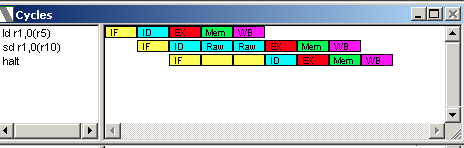
\includegraphics[scale=0.45]{forwarding-1.png}
\end{frame}

\begin{frame}[fragile]
\frametitle{Forwarding - Lectura seguida de escritura}
\begin{itemize}
\item Lectura seguida de Escritura
\begin{itemize}
\item Con el adelantamiento activo, cuando la instrucción \emph{ld} pasa la etapa \emph{MEM}, ya puede adelantar el operando
\item La instrucción \emph{sd} necesita el registro r1 en la etapa de \emph{MEM}
\item Por lo tanto ya no hay atascos RAW.
\end{itemize}
\end{itemize}
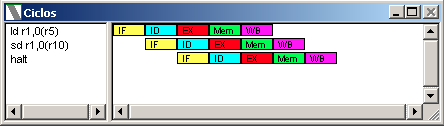
\includegraphics[scale=0.45]{forwarding-1-lectura-escritura.png}
\end{frame}


\begin{frame}[fragile]
\frametitle{Forwarding - Lectura seguida de Aritmetico / Logica}
\begin{itemize}
\item Lectura seguida de Aritmetico / Lógica
\begin{itemize}
\item Uno de los operandos de una instrucción aritmetico lógico proviene de una lectura de memoria
\item La instrucción \emph{daddi} debe esperar a que la instrucción \emph{ld} se complete, esperando en \emph{ID}
\end{itemize}
\end{itemize}
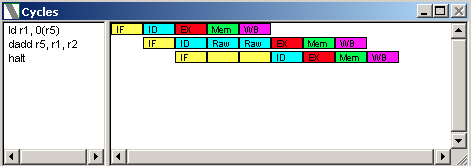
\includegraphics[scale=0.45]{forwarding-2.png}
\end{frame}

\begin{frame}[fragile]
\frametitle{Forwarding - Lectura seguida de Aritmetico / Logica}
\begin{itemize}
\item Lectura seguida de Aritmetico / Lógica
\begin{itemize}
\item Con el adelantamiento activo, cuando la instrucción \emph{ld} pasa la etapa \emph{MEM}, ya puede adelantar el operando
\item La instrucción \emph{daddi} necesita el registro r1 en la etapa de \emph{EX}
\item Como \emph{daddi} debe esperar en \emph{EX} a que \emph{ld} pase la etapa \emph{MEM}, se produce un solo atasco RAW.
\end{itemize}
\end{itemize}
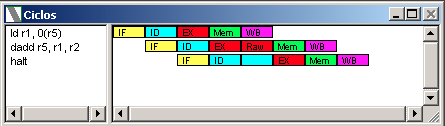
\includegraphics[scale=0.45]{forwarding-2-lectura-aritm.png}
\end{frame}


\begin{frame}[fragile]
\frametitle{Forwarding - Lectura seguida de Salto Condicional}
\begin{itemize}
\item Lectura seguida de Salto Condicional
\begin{itemize}
\item Uno de los operandos de una instrucción de salto condicional proviene de una lectura de memoria
\item La instrucción \emph{beqz} debe esperar a que la instrucción \emph{ld} se complete, esperando en \emph{ID}
\end{itemize}
\end{itemize}
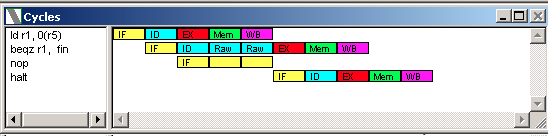
\includegraphics[scale=0.45]{forwarding-3.png}
\end{frame}

\begin{frame}[fragile]
\frametitle{Forwarding - Lectura seguida de Salto Condicional}
\begin{itemize}
\item Lectura seguida de Salto Condicional
\begin{itemize}
\item Con el adelantamiento activo, cuando la instrucción \emph{ld} pasa a la etapa \emph{MEM}, ya puede adelantar el operando
\item La instrucción \emph{beqz} necesita el registro r1 en la etapa de \emph{ID}
\item Por lo tanto esta situación no cambia
\end{itemize}
\end{itemize}
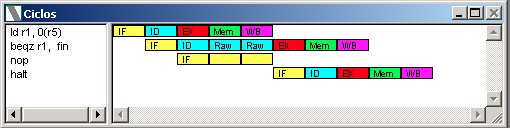
\includegraphics[scale=0.45]{forwarding-3-lectura-beq.png}
\end{frame}


\begin{frame}[fragile]
\frametitle{Forwarding - Aritmetica / Lógica seguida de Escritura}
\begin{itemize}
\item Aritmetica / Lógica seguida de Escritura
\begin{itemize}
\item El operando a escribir en memoria viene de una instrucción aritmetico lógica anterior.
\item La instrucción \emph{sd} debe esperar a que la instrucción \emph{daddi} se complete, esperando en \emph{ID}
\end{itemize}
\end{itemize}
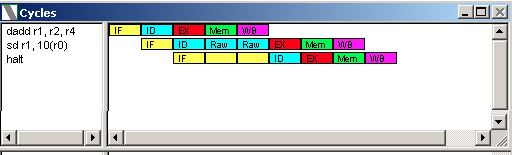
\includegraphics[scale=0.45]{forwarding-4.png}
\end{frame}

\begin{frame}[fragile]
\frametitle{Forwarding - Aritmetica / Lógica seguida de Escritura}
\begin{itemize}
\item Aritmetica / Lógica seguida de Escritura
\begin{itemize}
\item Con el adelantamiento activo, cuando la instrucción \emph{daddi} pasa la etapa \emph{EX}, ya puede adelantar el operando
\item La instrucción \emph{sd} necesita el registro r1 en la etapa de \emph{MEM}
\item Por lo tanto ya no hay atascos RAW.
\end{itemize}
\end{itemize}
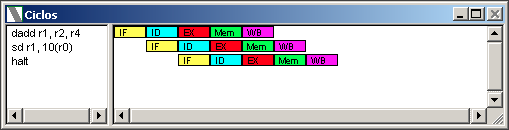
\includegraphics[scale=0.45]{forwarding-4-aritmetica-escritura.png}
\end{frame}

\begin{frame}[fragile]
\frametitle{Forwarding - Aritmetica / Lógica seguida de Aritmetico / Logica}
\begin{itemize}
\item Aritmetica / Lógica seguida de Aritmetico / Logica
\begin{itemize}
\item Un operando de una instrucción aritmetico lógica viene de una instrucción aritmetico lógica anterior.
\item La segunda  instrucción \emph{daddi} debe esperar a que la primer instrucción \emph{daddi} se complete, esperando en \emph{ID}
\end{itemize}
\end{itemize}
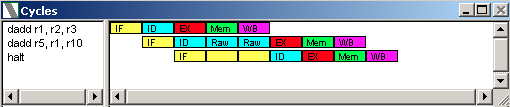
\includegraphics[scale=0.45]{forwarding-5.png}
\end{frame}

\begin{frame}[fragile]
\frametitle{Forwarding - Aritmetica / Lógica seguida de Aritmetico / Logica}
\begin{itemize}
\item Aritmetica / Lógica seguida de Aritmetico / Logica
\begin{itemize}
\item Con el adelantamiento activo, cuando la primer instrucción \emph{daddi} pasa la etapa \emph{EX}, ya puede adelantar el operando
\item La segunda instrucción \emph{daddi} necesita el registro r1 en la etapa de \emph{EX}
\item Por lo tanto ya no hay atascos RAW.
\end{itemize}
\end{itemize}
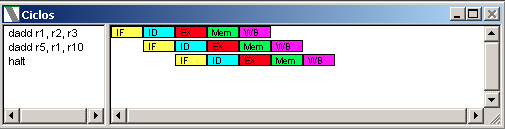
\includegraphics[scale=0.45]{forwarding-5-aritmetica-aritmetica.png}
\end{frame}


\begin{frame}[fragile]
\frametitle{Forwarding - Aritmetica / Lógica seguida de Salto Condicional}
\begin{itemize}
\item Aritmetica / Lógica seguida de Salto Condicional
\begin{itemize}
\item Un operando de una instrucción de salto condicional viene de una instrucción aritmetico lógica anterior.
\item La instrucción \emph{beqz} debe esperar a que la instrucción \emph{daddi} se complete, esperando en \emph{ID}
\end{itemize}
\end{itemize}
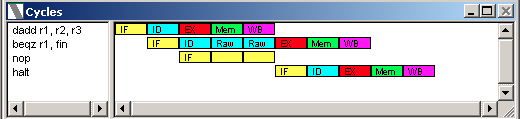
\includegraphics[scale=0.45]{forwarding-6.png}
\end{frame}

\begin{frame}[fragile]
\frametitle{Forwarding - Aritmetica / Lógica seguida de Salto Condicional}
\begin{itemize}
\item Aritmetica / Lógica seguida de Salto Condicional
\begin{itemize}
\item Con el adelantamiento activo, cuando la instrucción \emph{daddi} pasa la etapa \emph{EX}, ya puede adelantar el operando
\item La instrucción \emph{beqz} necesita el registro r1 en la etapa de \emph{ID}
\item Como \emph{beqz} debe esperar en \emph{ID} a que \emph{daddi} pase la etapa \emph{EX}, se produce un solo atasco RAW.
\end{itemize}
\end{itemize}
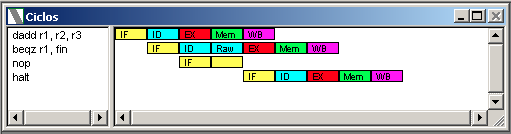
\includegraphics[scale=0.45]{forwarding-6-aritmetica-salto-condicional.png}
\end{frame}

\begin{frame}[fragile]
\frametitle{Forwarding - Lectura seguida de Lectura}
\begin{itemize}
\item Lectura seguida de Lectura
\begin{itemize}
\item El operando que calcula el desplazamiento en memoria de una escritura viene de una instrucción de lectura anterior.
\item La segunda instrucción \emph{ld} debe esperar a que la primer instrucción \emph{ld} se complete, esperando en \emph{ID}
\end{itemize}
\end{itemize}
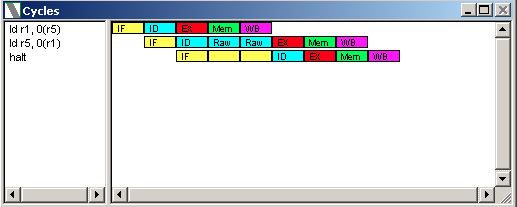
\includegraphics[scale=0.45]{forwarding-7.png}
\end{frame}

\begin{frame}[fragile]
\frametitle{Forwarding - Lectura seguida de Lectura}
\begin{itemize}
\item Lectura seguida de Lectura
\begin{itemize}
\item Con el adelantamiento activo, cuando la primer instrucción \emph{ld} pasa la etapa \emph{MEM}, ya puede adelantar el operando
\item La segunda instrucción \emph{ld} necesita acceder a r1 en la etapa \emph{EX}
\item Como la segunda instrucción \emph{ld} debe esperar en \emph{EX} a que la primer instrucción  \emph{ld} pase la etapa \emph{MEM}, se produce un solo atasco RAW.

\end{itemize}
\end{itemize}
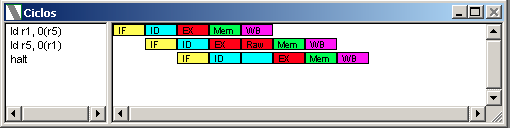
\includegraphics[scale=0.45]{forwarding-7-lectura-lectura.png}
\end{frame}


\begin{frame}[fragile]
\frametitle{Forwarding - Aritmetica / Lógica seguida de Lectura}
\begin{itemize}
\item Aritmetica / Lógica seguida de Lectura
\begin{itemize}
\item El operando que calcula el desplazamiento en memoria de una escritura viene de una instrucción aritmetico lógica anterior.
\item La instrucción \emph{ld} debe esperar a que la instrucción \emph{daddi} se complete, esperando en \emph{ID}
\end{itemize}
\end{itemize}
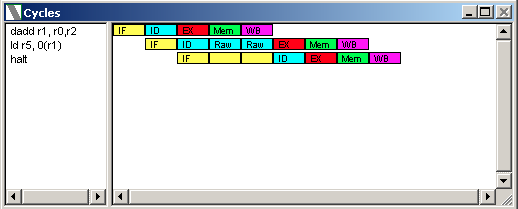
\includegraphics[scale=0.45]{forwarding-8.png}
\end{frame}

\begin{frame}[fragile]
\frametitle{Forwarding - Aritmetica / Lógica seguida de Lectura}
\begin{itemize}
\item Aritmetica / Lógica seguida de Lectura
\begin{itemize}
\item Con el adelantamiento activo, cuando la instrucción \emph{daddi} pasa la etapa \emph{EX}, ya puede adelantar el operando
\item La instrucción \emph{ld} necesita acceder a r1 en la etapa \emph{EX}
\item Por lo tanto ya no hay atascos RAW.
\end{itemize}
\end{itemize}
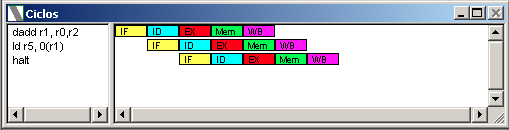
\includegraphics[scale=0.45]{forwarding-8-aritmetica-lectura.png}
\end{frame}

\end{document}

